\chapter{Testing and Evaluation}

To answer our research question of how to improve the performance of Web
services in DIL environments, we developed some test scenarios. In this chapter
we present how the testing was performed and then present the results we
obtained.

\section{Test Scenarios}
\begin{enumerate}
    \item REST-client and server sending each other GET requests.
    \item W3c Web services.
\end{enumerate}

Both the REST and Web service applications were developed with Java.

\subsection{Using proxies}

In order to enable the applications to tunnel all their HTTP traffic through our
proxy, we needed a way to setup a proxy without altering the applications
themselves. Fortunately, Java provide mechanisms to deal with
proxies\cite{oracle-proxy}. We configured the \gls{jvm} to get the applications
to tunnel all HTTP traffic through our proxy. This is done by setting properties
to the \gls{jvm}:


\begin{lstlisting}[frame=single, caption="Setting a proxy on the \gls{jvm}", label=test]
java -Dhttp.proxyHost=localhost \
-Dhttp.proxyPort=3001 \
-Dhttp.nonProxyHosts= \
-jar target/client.jar
\end{lstlisting}

In \cref{test} the application \textbf{client.jar} is started and all HTTP
traffic will go through the proxy server at localhost on port 3001.


\section{\glsentrylong{netem}}

In order to simulate \gls{dil} environments we need some way to control the
properties of the network traffic. Fortunately, the Linux kernel offers a rich
set of tools for managing and manipulating the transmission of packets.

%Siter tldp -> Traffic Control HOWTO

\gls{netem} is an enchancement of the traffic control facilities that allows us
to control delay, packet loss and other characteristics to packets outgoing from
a selected network interface.
%Siter man-page om tc-netem

\subsection{NetEm emulating}

\textbf{tc}(traffic control) is a linux program to configure and control the
linux kernels Network scheduler.

\subsubsection{Delays}

NetEm can emulate delays on packets on a specific link.

\begin{lstlisting}[frame=single, caption="Emulating delay"]
  tc qdisc add dev eth0 root netem delay 100ms
\end{lstlisting}

In this example we add a fixed delay on 100 ms to all packets going out of local
Ethernet.

\section{Testing environment}

The majority of testing was performed on machines located at the FFI-lab at
Kjeller. Although testing on regular machines gives us a indication, to get as
realistic results as possible we also performed tests on military communication
equipment.

\subsection{Testing on computers}

 The Web service and client are connected to each other through a third
 computer, acting as a router. This machine have two network cards and will
 receive and forward IP packets from the client and Web service. The machines
 are networked together by Ethernet cables.

\begin{figure}[h]
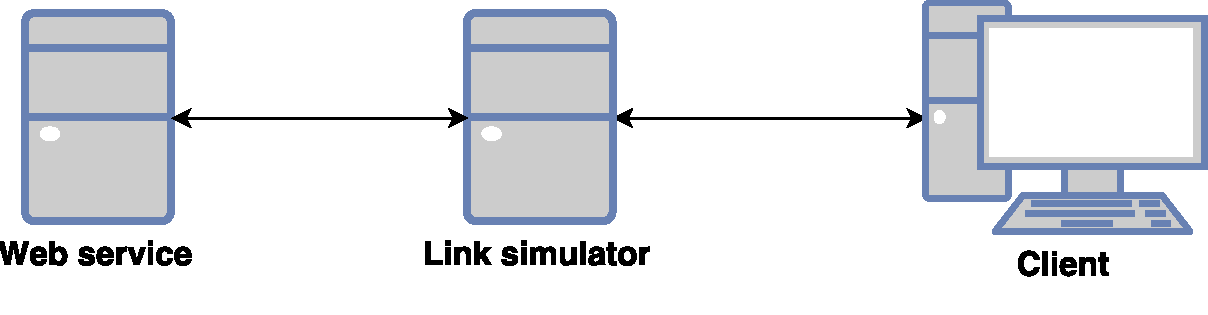
\includegraphics[scale=0.6]{images/testing_environment.pdf}
\caption{Testing environment}
\label{figure-testing-environment}
\end{figure}

\paragraph{Configuration}

This section describes how the test setup was performed. The computers running
the client and Web service are connect by an Ethernet cable to the "routing"
machine. Then they are assigned an IP address. This is done by the Linux network
interface administration program \textit{ifconfig}. In \cref{listing-ifconfig}
the Ethernet interface is assigned the IP address 192.168.2.3.

\begin{lstlisting}[frame=single, caption="Configuring a network interface", label=listing-ifconfig]
ifconfig eth0 192.168.2.3 up

\end{lstlisting}


\subsection{Testing on real hardware}
Kongsberg radio.


\section{Evaluation Tools}

\section{Test results}

In this section the results from the tests are presented. These results lead up to the discussion and conclusion in the next chapter.
